\section{Simulazioni PIL}
In questa sezione viene descritta brevemente la procedura per effettuare la simulazione PIL, i risultati ottenuti e i problemi riscontrati nell'impostare l'ambiente di simulazione.

Nella documentazione online di PX4, \cite{PIL}, dove erroneamente si definisce Hardware In The Loop (HITL) la simulazione PIL, viene presentato lo schema di collegamento per effettuare questo tipo di simulazione, Figura (\ref{fig:PIL}).

\begin{figure}
	\centering
	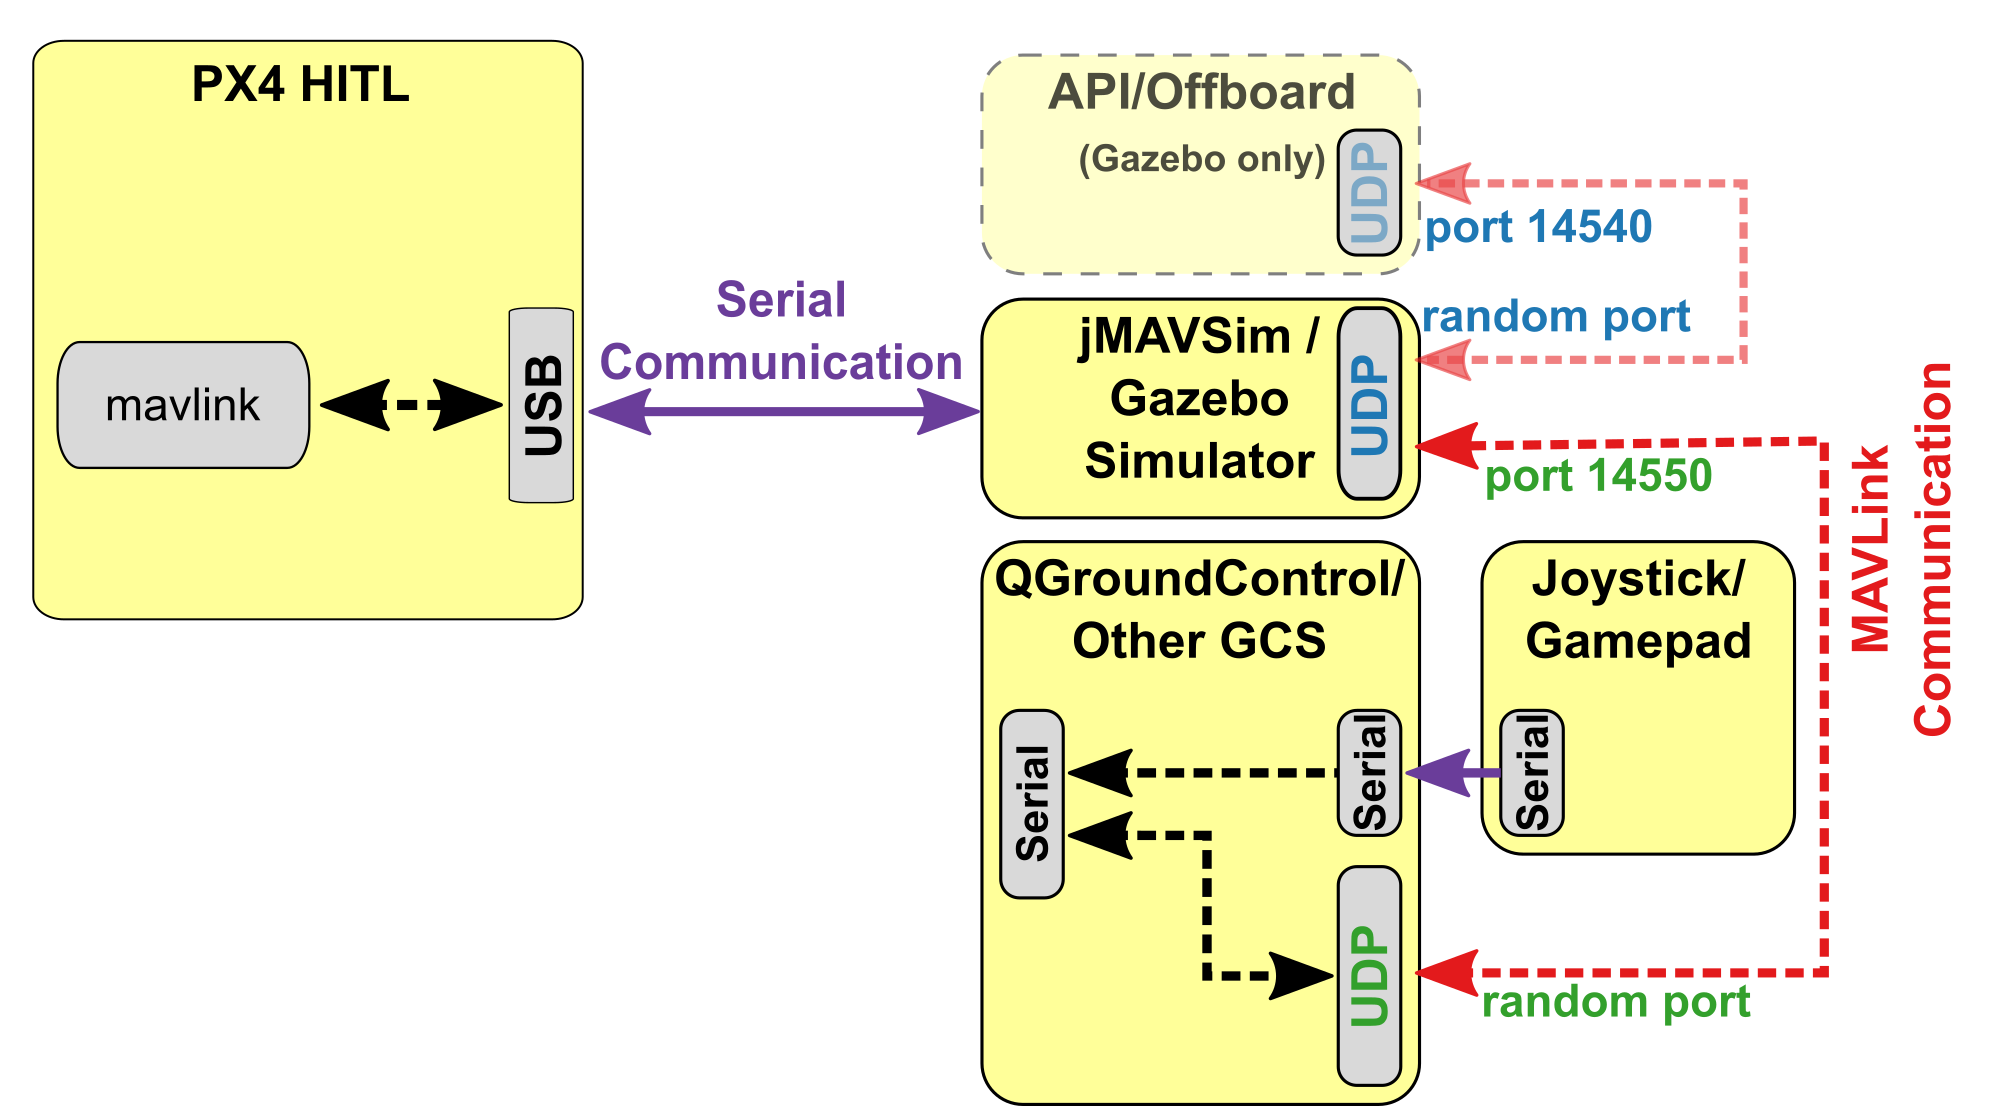
\includegraphics[width=0.6\textwidth]{Simulazioni/Figure/PIL}
	\caption{Schema di collegamento per la simulazione PIL, \cite{PIL}}
	\label{fig:PIL}
\end{figure}

Nella stessa guida sono presentate le impostazioni di Gazebo necessarie per questo tipo di simulazione.

Per utilizzare Simulink attraverso il tool "Embeded Coder Support Package for PX4 Autopilots", è necessaria la connessione tramite l'interfaccia USB per poter correttamente compilare, caricare ed eseguire il codice nell'hardware e salvare i dati della simulazione, \cite{PX4MATLAB}. Questo però non permette di rispettare il tipo di collegamento presentato nella Figura (\ref{fig:PIL}). 

Questo problema è stato aggirato modificando la procedura di boot del firmware scrivendo uno script di avvio personalizzato, e il settaggio del modulo di collegamento presente nella cartella di "Tools/sitl\_gazebo", allegato in Appendice. In questo modo viene settato un canale di connessione attraverso una porta seriale per comunicare con i sensori emulati in Gazebo, lasciando libera la porta USB per comunicare con Simulink. Non è stato possibile invece riuscire a trasportare il segnale PWM attraverso la stessa porta. Questo probabilmente perché la logica di funzionamento del sistema di controllo generato attraverso il Coder di Simulink non è coerente con il normale funzionamento del firmware PX4, che teoricamente dovrebbe trasportare questo genere di messaggi in modo automatico. No nè stato possibile quindi completare il settaggio necessario per effettuare le simulazioni PIL.
